\chapter{Transformer Networks}
\label{ch-transformer}

The primary reference for this chapter is  Ref.\cite{attention-is-all-you-need}.
Ref.\cite{attention-is-all-you-need} is  
 the highly influential  2017 paper entitled
``Attention is all you need" 
that introduced {\bf Transformer Networks} (TNs) and 
Attention into the AI vernacular.
Besides Ref.\cite{attention-is-all-you-need},
I also read blog posts
such as Ref.\cite{joshi-trans}
and the Wikipedia article on  TN (Ref. \cite{wiki-transformer}).
For a complete list of the large number
of excellent blog post that I read to learn
this subject, see my open source software texnn
(Ref.\cite{texnn}).\footnote{
texnn is
 Python software 
 that I wrote
specifically for drawing the bnets
of this chapter, but later I 
generalized it to a stand-alone app that can draw
any bnet (including SCMs, NNs and TNs), not just a TN bnet.}

Transformer Networks (TN)
have been taking the fields of
Natural Language Processing (NLP)
and Large Language Models (LLM)
by storm in recent years.
They were introduced in 2017 and already
are the basis of numerous LLMs.
For example,
BERT (Bidirectional Encoder
Representations from Transformers)
and ChatGPT (Generative Pre-trained Transformer),
two TN libraries that
have been trained with
huge databases such as all of
English Wikipedia (2,500M words).

How well ChatGPT works was a huge
surprise to most people, including experts in AI/ML.
My conjecture is that this surprising
LLM performance is
 due to causality.
 Let me explain. I believe TNs and the LLM that use them, are just curve-fitters (so are Least Squares, vanilla NNs, Convolutional NNs, etc.). But, we lucked out, because
TNs are very good at fitting causal data, and the space of all human generated text, including math
equations and computer code,
is causality connected (i.e., has
a {\bf causally connected topology}.).

Normally, TNs are
drawn as box diagrams
that are somewhat cryptic and ambiguous, at least to me.
In this chapter,
instead of 
drawing them as box diagrams,
I represent them as causal DAGs (bnets). This makes their
causal nature more explicit than 
the box diagrams, and,
in my opinion, also makes them
less ambiguous  and more understandable than the box diagrams.




Recurrent Neural Nets (RNNs)
are discussed in Chapter \ref{ch-rnn}.
TNs are quickly displacing RNNs, 
an older method, in NLP.  TNs are better than RNNs 
for doing NLP in several important ways. Whereas
 RNNs analyze the tokens (words) of a sentence 
sequentially (like a Kalman Filter), 
TNs analyze them in parallel, and thus are more
 amenable to parallel computing. Also, because
 RNNs analyze the words of a sentence sequentially, 
they tend to give more importance to the end 
of a sentence than to its beginning. That's because 
RNNs start forgetting the beginning of a sentence
 by the time they reach its end, like a patient 
with Alzheimer's. TNs do not suffer from this malady.

Dynamical bnets are discussed in Chapter \ref{ch-dyn-bnet}.
In Chapter \ref{ch-rnn},
we showed that RNNs
are dynamical bnets.
In this chapter
 we will show that TNs
dynamical bnets too.


In this chapter, we 
will use the Numpy-like tensor notation
discussed in Section 
\ref{sec-numpy-tensors}. In particular, note that $[n] = [0:n] = \{0, 1,\ldots, n-1\}$ and that $T^{[n], [m]}$ is an $n\times m$ matrix.

\section{Recurrent Neural Net with Attention}
\subsection{Single Head Attention}

Let

$\ell$ be the maximum number of words allowed in a sentence.
Some words might be blanks (padding).

$e_\alp^t\in \RR^{d}$ be
a $d$ dimensional column vector
for word $\alp\in [\ell]$ at time $t$.

$W_\rvq^t, W_\rvk^t, W_\rvv^t\in \RR^{d\times d}$
be the  weight matrices for time
slice $t$.
These matrices are learned by training
the net.
The letters $Q,K,V$ stand for
 Query, Key and Value,
respectively.
They transform $e_\alp^t$ 
as follows

\beq
\left\{
\begin{array}{l}
v_\alp^t = W_\rvv^t e_\alp^t
\\
q_\alp^t = W_\rvq^t e_\alp^t
\\
k_\alp^t = W_\rvk^t e_\alp^t
\end{array}
\right.
\eeq



\begin{figure}[h!]\centering
$$\xymatrix@C=4pc{
&{\underline{v_0^t}}\ar[dr]\ar[ddddr]\ar[dddddddr]&
\\
{\underline{e_0^t}}\ar[dr]_{W_{\rvk}^t}\ar@[red][r]^{W_{\rvq}^t}\ar[ur]^{W_{\rvv}^t}&{\underline{q_0^t}}\ar@[red][r]&{\underline{e_0^{t+1}}}
\\
&{\underline{k_0^t}}\ar[ur]\ar[ddr]\ar[dddddr]&
\\
&{\underline{v_1^t}}\ar[uur]\ar[dr]\ar[ddddr]&
\\
{\underline{e_1^t}}\ar[dr]_{W_{\rvk}^t}\ar@[red][r]^{W_{\rvq}^t}\ar[ur]^{W_{\rvv}^t}&{\underline{q_1^t}}\ar@[red][r]&{\underline{e_1^{t+1}}}
\\
&{\underline{k_1^t}}\ar[uuuur]\ar[ur]\ar[ddr]&
\\
&{\underline{v_2^t}}\ar[uuuuur]\ar[uur]\ar[dr]&
\\
{\underline{e_2^t}}\ar[dr]_{W_{\rvk}^t}\ar@[red][r]^{W_{\rvq}^t}\ar[ur]^{W_{\rvv}^t}&{\underline{q_2^t}}\ar@[red][r]&{\underline{e_2^{t+1}}}
\\
&{\underline{k_2^t}}\ar[uuuuuuur]\ar[uuuur]\ar[ur]&
\save
\POS"2,1"."8,1"."2,1"."8,1"!C*+<1.0em>\frm{--}
\POS"1,2"."3,2"."1,3"."3,3"!C*+<1.5em>\frm{--}
\POS"4,2"."6,2"."4,3"."6,3"!C*+<1.5em>\frm{--}
\POS"7,2"."9,2"."7,3"."9,3"!C*+<1.5em>\frm{--}
\restore
}$$
\caption{Recurrent single-head attention for 3 words. Time-slice $t$
of dynamical bnet for
 a transformer network (TN)
of a 3-word sentence.
Note that $k_\alp^t$
for all $\alp$
points to $\rve^{t+1}_\beta$ for all $\beta\in[\ell]$.
Likewise,
$\rvv_\alp^t$
for all $\alp$
points to $\rve^{t+1}_\beta$ for all $\beta\in [\ell]$.
However, 
$\rvq_\alp^t$
points only to $\rve^{t+1}_\alp$.
}
\label{fig-transformer-full-3-word}
\end{figure}

Fig.\ref{fig-transformer}
represents a TN 
of a 3-word sentence as a dynamical bnet.
The TPMs,
printed in blue,
for bnet
Fig.\ref{fig-transformer},
are as follows:

\beq\color{blue}
P(v_\alp^t|e_\alp^t)=
\indi(\;\;\;
v_\alp^t = W_\rvv^t e_\alp^t
\;\;\;)
\eeq

\beq\color{blue}
P(q_\alp^t|e_\alp^t)=
\indi(\;\;\;
q_\alp^t = W_\rvq^t e_\alp^t
\;\;\;)
\eeq

\beq\color{blue}
P(k_\alp^t|e_\alp^t)=
\indi(\;\;\;
k_\alp^t= W_\rvk^t e_\alp^t
\;\;\;)
\eeq

\beq\color{blue}
P(e^{t+1}_\alp|v_.^t,q_\alp^t,
 k_.^t)
=
\indi(\;\;\;
e_\alp^{t+1}=
\sum_{\beta\in[\ell]}
v_\beta^t
P(\beta|q_\alp^t)
\;\;)
\label{eq-attention-average}
\eeq
where the conditional
probability 
$P(\beta|q_\alp^t)$ is 
called defined as

\beqa
P(\beta|q_\alp^t)&=&
\softmax((q_\alp^t)^T k_\beta^t)(\beta)
\\
&=&
\frac{e^{(q_\alp^t)^T k_\beta^t}}
{\sum_{\beta'\in [\ell]}
e^{(q_\alp^t)^T k_{\beta'}^t}}
\eeqa

The right hand side of Eq.(\ref{eq-attention-average})
constitutes an average over 
all the word vectors $\{\rvv_\alp^t: \alp\in[\ell]\}$
in a sentence.
This average, 
or the conditional
probability $P(\beta|q_\alp^t)$,
are called an {\bf Attention}.




On first encounter, the structure of a TN
seems a bit mysterious. Then one realizes that this is
an old friend. 
If the dashed  boxes in 
Fig.\ref{fig-transformer-full-3-word} are each ``shrunk" to single nodes,
then it becomes a TAN Bayes Net. Each of the 3 subgraphs $\rve^t, (\rvv^t, \rvq^t, \rvk^t), \rve^{t+1} $
also constitutes a TAN Bayes net. \footnote{Tree Augmented Naive (TAN) Bayes nets
were introduced in Chapter \ref{ch-chow}}.\footnote{A {\bf reverse or upside down tree} is obtained by reversing the directions of all the arrows of a tree directed graph. A TAN Bayes net is normally defined as in Chapter\ref{ch-chow}, as a Naive Bayes net augmented with a tree. In transformers, the Naive Bayes Net is augmented with a reverse tree (RT) instead of a tree (T), so technically transformers contain RTAN (or simply AN) Bayes nets, not TAN Bayes nets. }
In broad terms, Fig.\ref{fig-transformer-full-3-word}
can be described by saying that
each word undergoes a special
kind of 3-class (q,k,v) Naive Bayes
classification,
and the results of that classification
are sent to the new version of each word (except the q class which only sends
info to one word, not all of them).






\begin{figure}[h!]\centering
$$\xymatrix@R=4pc@C=4pc{
&{\underline{(k^t)}^{[d],[\ell]}}\ar[dr]&
\\
{\underline{(e^t)}^{[d],[\ell]}}\ar[ur]^{W_\rvk^{[d], [d]}}\ar@[red][r]^{W_\rvq^{[d], [d]}}\ar[dr]_{W_\rvv^{[d], [d]}}&{\underline{(q^t)}^{[d],[\ell]}}\ar@[red][r]&{\underline{(e^{t+1})}^{[d],[\ell]}}
\\
&{\underline{(v^t)}^{[d],[\ell]}}\ar[ur]&
}$$
\caption{Recurrent single-head attention for $\ell=3$ words. Folded. Note that the  input $e^t$ and the output $e^{t+1}$ have the same shape.}
\label{fig-texnn-for-transformer-recurrent-3-words-folded}
\end{figure}

\begin{subequations}

\begin{equation}\color{blue}
(e^t)^{[d],[\ell]} = \;\;\text{prior}
\label{eq-A-fun-transformer-recurrent-3-words-folded}
\end{equation}

\begin{equation}\color{blue}
(e^{t+1})^{[d],[\ell]} = \text{Attention}((v^t)^{[d],[\ell]},(q^t)^{[d],[\ell]},(k^t)^{[d],[\ell]})
\label{eq-X-fun-transformer-recurrent-3-words-folded}
\end{equation}

\begin{equation}\color{blue}
(k^t)^{[d],[\ell]} = W_\rvk^{[d], [d]} (e^t)^{[d],[\ell]}
\label{eq-K-fun-transformer-recurrent-3-words-folded}
\end{equation}

\begin{equation}\color{blue}
(q^t)^{[d],[\ell]} = W_\rvq^{[d], [d]} (e^t)^{[d],[\ell]}
\label{eq-Q-fun-transformer-recurrent-3-words-folded}
\end{equation}

\begin{equation}\color{blue}
(v^t)^{[d],[\ell]} = W_\rvv^{[d], [d]} (e^t)^{[d],[\ell]}
\label{eq-V-fun-transformer-recurrent-3-words-folded}
\end{equation}

\end{subequations}


\subsection{Multi-Head Attention}

\begin{figure}[h!]\centering
$$\xymatrix@R=4pc@C=4pc{
&{\underline{(k^t)}^{[D],[\ell]}}\ar[dr]&
\\
{\underline{(e^t)}^{[d],[\ell]}}\ar[ur]^{W_\rvk^{[D], [d]}}\ar@[red][r]^{W_\rvq^{[D], [d]}}\ar[dr]_{W_\rvv^{[D], [d]}}&{\underline{(q^t)}^{[D],[\ell]}}\ar@[red][r]&{\underline{(e^{t+1})}^{[d],[\ell]}}
\\
&{\underline{(v^t)}^{[D],[\ell]}}\ar[ur]&
}$$
\caption{Recurrent single-head attention for $\ell=3$ words. Folded. Note that the  input $e^t$ and the output $e^{t+1}$ have the same shape $([d], [\ell])$.}
\label{fig-texnn-for-transformer-recurrent-3-words-folded-multi-head}
\end{figure}

\begin{subequations}

\begin{equation}\color{blue}
(e^t)^{[d],[\ell]} = \;\;\text{prior}
\label{eq-A-fun-transformer-recurrent-3-words-folded-multi-head}
\end{equation}

\begin{equation}\color{blue}
(e^{t+1})^{[d],[\ell]} = \text{Multi-Head-Attention}((v^t)^{[D],[\ell]},(q^t)^{[D],[\ell]},(k^t)^{[D],[\ell]})
\label{eq-X-fun-transformer-recurrent-3-words-folded-multi-head}
\end{equation}

\begin{equation}\color{blue}
(k^t)^{[D],[\ell]} = W_\rvk^{[D], [d]} (e^t)^{[d],[\ell]}
\label{eq-K-fun-transformer-recurrent-3-words-folded-multi-head}
\end{equation}

\begin{equation}\color{blue}
(q^t)^{[D],[\ell]} = W_\rvq^{[D], [d]} (e^t)^{[d],[\ell]}
\label{eq-Q-fun-transformer-recurrent-3-words-folded-multi-head}
\end{equation}

\begin{equation}\color{blue}
(v^t)^{[D],[\ell]} = W_\rvv^{[D], [d]} (e^t)^{[d],[\ell]}
\label{eq-V-fun-transformer-recurrent-3-words-folded-multi-head}
\end{equation}

\end{subequations}


\section{Vanilla TN}

\begin{figure}[h!]
\centering
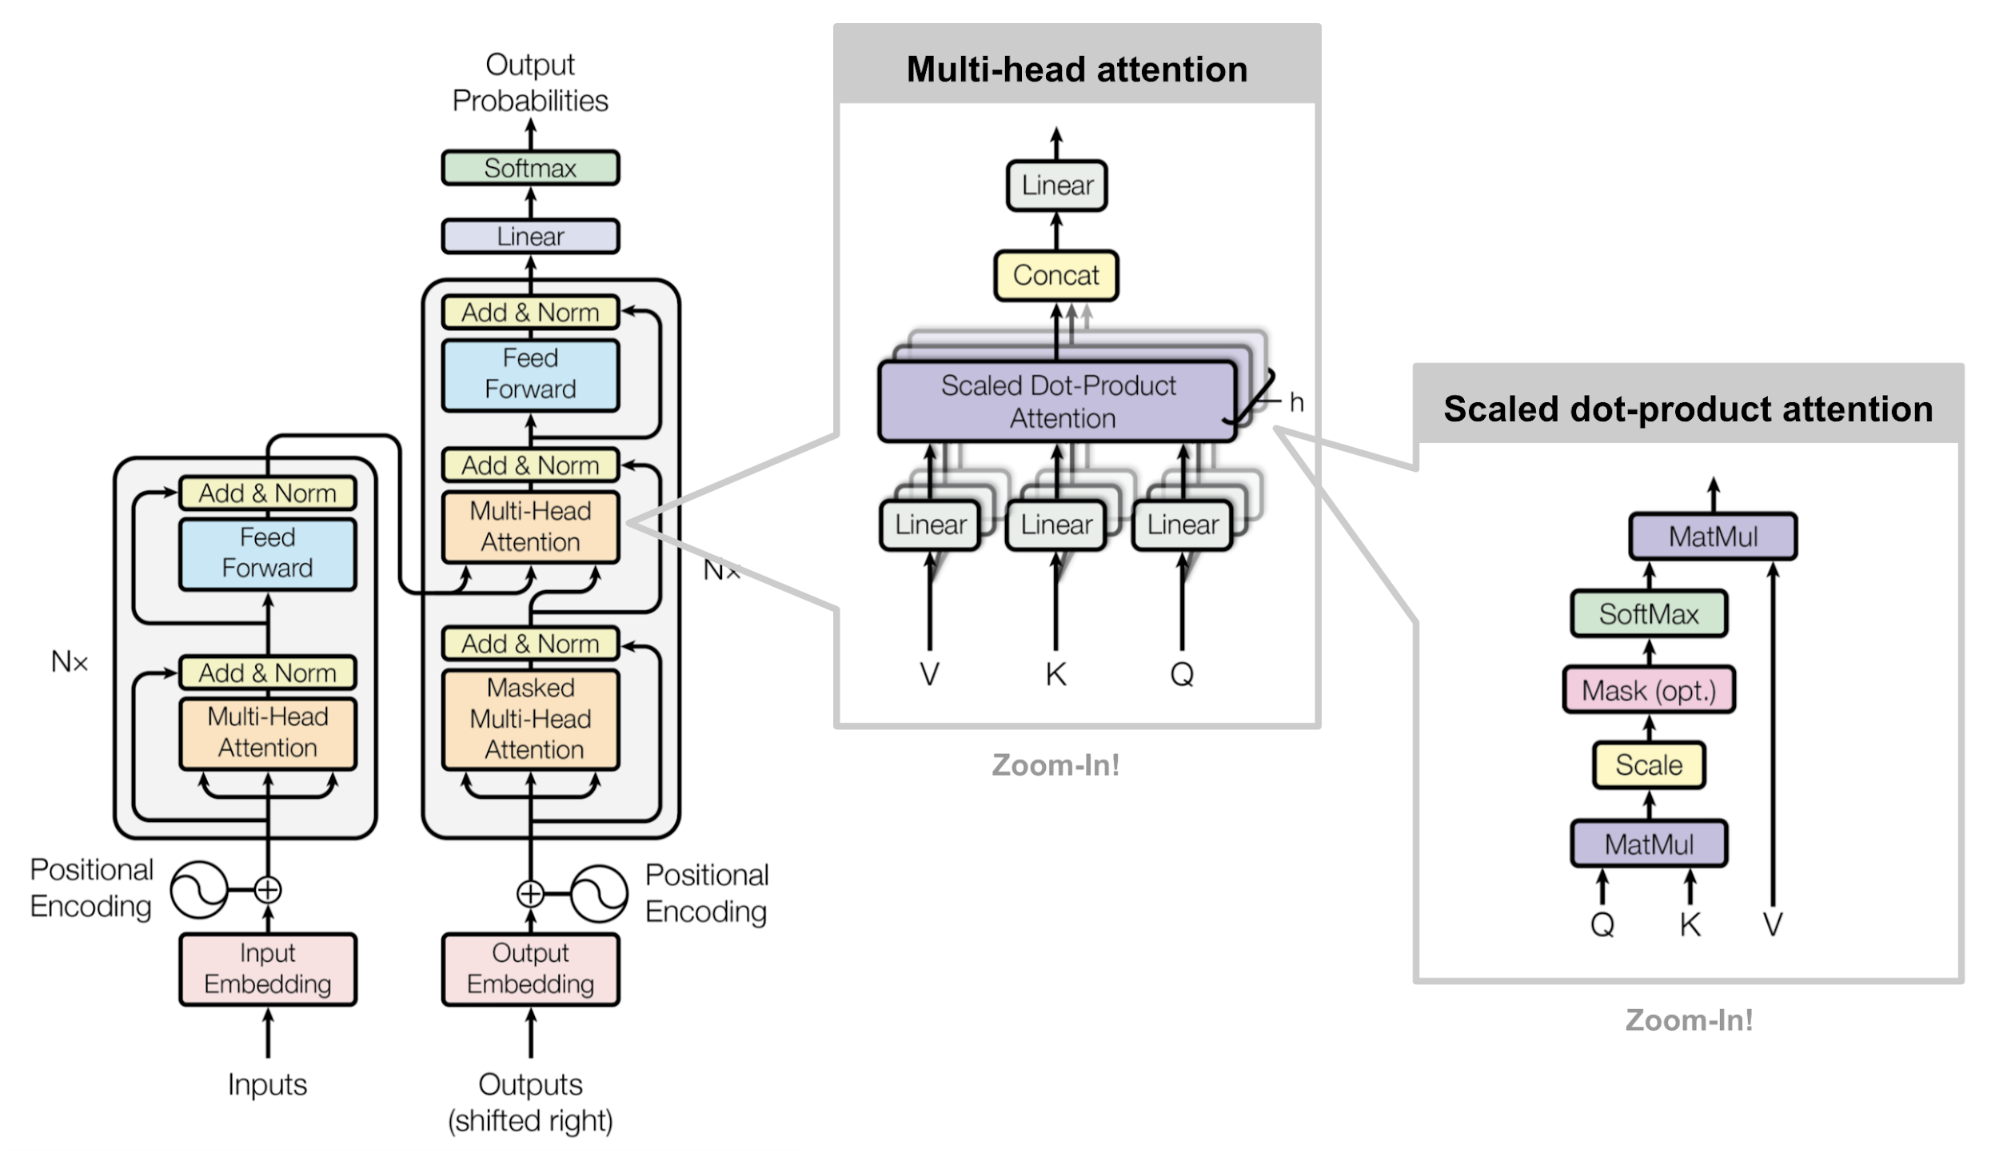
\includegraphics[width=6in]
{transformer/transformer.png}
\caption{Vanilla Transformer}
\label{fig-vanilla-transformer}
\end{figure}

Our tensor notation is discussed in Section 
\ref{sec-numpy-tensors} of Bayesuvius.


$\ell=$ maximum number of words in a sentence segment. $\alp\in [\ell]$, $\ell\sim 100$

$L=$ number of words in vocabulary, $\beta\in[L]$, $L>> \ell$

$d=d_\rvq=d_\rvk=d_\rvv=64$, hidden dimension  per head,
$\delta\in[d]$. 

$n_\rvh=8$, number of heads, $\nu \in[n_\rvh]$

$D=n_\rvh d=8(64)=512$, hidden dimension for all heads,
$\Delta\in [D]$

$\Lambda=6$, number of layers in plate (a.k.a., stack), $\lam\in[\Lambda]$

reshaping
\beq
T^{\nu, \delta}\rarrow T^{\Delta}
\;\;
\left(
T^{[n_\rvh], [d]} \rarrow T^{[D]}
\right)
\eeq

\beq
T^{\Delta}\rarrow T^{\nu, \delta}
\;\;
\left(
T^{[D]}\rarrow T^{[n_\rvh], [d]}
\right)
\eeq

concatenation
\beq
T^{[n]}= (T^0, T^1,\ldots, T^{n-1})= 
(T^\nu)_{\nu\in[n]}
\eeq

Hadamard product (element-wise, entry-wise multiplication)
\beq
T^{[n]}* S^{[n]}= (T^\nu S^\nu)_{\nu\in[n]}
\eeq


Matrix multiplication
( $T^{[n]}= T^{[n], [1]}$ is a column vector)

\beq
(T^{[n]})^T S^{[n]}=\text{scalar}
\eeq

\beq
T^{[a],[b]}S^{[b], [c]}
=\left[\sum_{\beta\in[b]} T^{\alp, \beta}
S^{\beta, \gamma}\right]
_{\alp_\in [a], \gamma \in [c]}
\eeq

Most treatments of TN, including the
``Transformers is All You Need paper",  order the
operations chronologically from
left to right. So if $A$ occurs before $B$,
they write $AB$.
This is contrary 
to what is done in Linear Algebra, where one 
orders the operations chronologically from right to left, and one writes $BA$.
We will adhere to the Linear Algebra
convention, since it is so prevalent
and is the overwhelming precedent.


\beq
e^{\beta, \alp} =\delta(\beta, \beta(\alp))
\left(
e^{[L], [\ell]} \text{ has one hot columns.}
\right)
\eeq


{\bf Embedding (a.k.a. encoding) Matrix}
\beq
e^{\delta, \alp} = \sum_\beta 
E^{\delta, \beta}
e^{\beta, \alp}
\;\;
\left(
e^{[d],[\ell]}= E^{[d], [L]}e^{[L], [\ell]}
\right)
\eeq

{\bf Weight matrices}

\beq
Q^{\nu,\delta, \alp}=\sum_{\delta'}
W_\rvq^{\nu, \delta, \delta'}e^{\delta', \alp}
\;\;
\left(
Q^{[D], [\ell]}=
W_\rvq^{[D],[d]}E^{[d],[\ell]}
\right)
\eeq


\beq
K^{\nu,\delta, \alp}=
\sum_{\delta'}
W_\rvk^{\nu, \delta, \delta'}
e^{\delta', \alp}
\;\;
\left(
K^{[D], [\ell]}=
W_\rvk^{[D],[d]}E^{[d],[\ell]}
\right)
\eeq

\beq
V^{\nu,\delta, \alp}=
\sum_{\delta'}
W_\rvv^{\nu, \delta, \delta'}
e^{\delta', \alp}
\;\;
\left(
V^{[D], [\ell]}=
W_\rvv^{[D],[d]}E^{[d],[\ell]}
\right)
\eeq



\beq
B^{
\nu,\alp, \alp'}=
\frac{1}{\sqrt{d}}
\sum_\delta K^{\nu,\delta,\alp}
Q^{\nu,\delta,\alp'}
\;\;
\left(
B^{[n_h],[\ell],[\ell]}
=\left[
\frac{1}{\sqrt{d}}
(K^{\nu, [d], [\ell]})^T
Q^{\nu, [d], [\ell]}\right]_{\nu\in[n_\rvh]}
\right)
\eeq

\beqa
A^{\nu, 
\delta, \alp'}&=&
\sum_{\alp}
V^{\nu, \delta, \alp}
\underbrace{
{\rm softmax}(B^{\nu, \alp ,\alp'})}_{
P(\alp|\nu, \alp')}
\eeqa

\beq
\sum_{\alp\in [\ell]}P(\alp|\nu, \alp')=1
\eeq

\beq
A^{\nu, \delta, \alp'}
\rarrow
A^{\Delta, \alp'}
\left(
A^{[n_\rvh], [d], [\ell]}
\rarrow
A^{[D], [\ell]}\right)
\eeq

Column vector notation:

\beq
B^{\nu, \alp, \alp'}=
\frac{1}{\sqrt{d}}
(K^{\nu, [d], \alp})^T Q^{\nu, [d], \alp'}
\eeq
Important: Note that the softmax() makes the
$\alp$ component a probability,
not the $\alp'$ one!

For example, suppose $\nu=1$ (one head), $\ell=2$ (a 2 word segment), 
and $d=3$ (hidden dimension is 3).
The $Q^{[3], [2]}, K^{[3], [2]}, V^{[3], [2]}$ are $3\times 2$ matrices
(i.e, 2 3-dim column vectors).
One uses the $Q^{[3], [2]}$ and $K^{[3], [2]}$ to arrive at a 
$2\times 2$ matrix $P(\alp'|\alp)$
of probabilities.
Then one uses that matrix of probabilities to replace

\beq
\left[
V^{[3], 0}, V^{[3], 1} 
\right]
\rarrow
\left[
V^{[3], 0} P(0|0)
+ 
V^{[3], 1}P(1|0)
,
V^{[3], 0} P(0|1)
+ 
V^{[3], 1}P(1|1)
\right]
\eeq

\begin{itemize}
\item{\bf Positional Embedding Matrix}
 
$E_{pos}^{[d],[\ell]}$

\beq
E_{pos}^{\delta, \beta}=
\left\{
\begin{array}{ll}
\sin\left(\frac{\beta}
{10^{4\delta/d}}\right)= \sin(2\pi \frac{\beta}{\lam(\delta)})
& \text{if $\delta$ is even}
\\
\cos\left(\frac{\beta}{10^{4(\delta-1)/d}}\right)=
\cos(2\pi\frac{\beta}{\lam(\delta)})
& \text{if $\delta$ is odd}
\end{array}
\right.
\eeq
$E_{pos}^{\delta, \beta}$ changes in phase by $\pi/2$  
every time $\delta$ changes by 1. Its wavelength 
$\lam$ is independent
of $\beta$, but increases rapidly with $\delta$, from $\lam(\delta=0)=2\pi*1$ to 
$\lam(\delta=d)= 2\pi* 10^4$.

Total Embedding equals initial embedding plus 
positional embedding:$E = E_0 + E_{pos}$


The purpose of positional embedding is to take $e^{\beta, \alp}$ to $e^{\delta, \alp}=
\sum_\beta E^{\delta,\beta}_{pos} e^{\beta, \alp}$
where $e^{\delta, \alp}$ changes quickly as $\delta$ (i.e., position) changes.

\item {\bf ReLU}

For a tensor $T$ of arbitrary shape
\beq
ReLU(T) = (T)_+ = max(0, T)
\eeq
max element-wise

\item {\bf Feed Forward neural net}
\beq
F(e^{[1], [\ell]}) = ReLU(e^{[1],[\ell]}
W_1^{[\ell], [d]} + b_1^{[1],[d]}) W_2^{[d], [\ell]} + b_1^{[1],[\ell]}
\eeq

\beq
F(e^{[\ell]}) = W_2^{[\ell], [d]}ReLU(
W_1^{[d], [\ell]}e^{[\ell]} + b_1^{[d]})  + b_1^{[\ell]}
\eeq

\item {\bf Softmax}

softmax() takes a vector and returns
a vector of probabilities of the same length

\beq
e^{[n]}\rarrow P^{[n]}
\eeq
where

\beq
P^\alp=
\frac{\exp(e^\alp)}
{\sum_{\alp\in[n]} \exp(e^\alp )}
\;\;
\left(P^{[n]}=\frac{\exp(e^{[n]})}
{\norm{\exp(e^{[n]})
}_0}
\right)
\eeq

For example,
\beq
(1,0,0)\rarrow (e,1,1)/norm
\eeq

\beq
(10,0,0)\rarrow (e^{10}, 1, 1)/norm \approx (1,0,0)
\eeq

For any $a\in\RR$,
\beq
(a,a,a)\rarrow (1, 1, 1)/3
\eeq


\item {\bf Skip Connection (Add \& Normalize)}

A {\bf skip connection} is when you split the
input to a {\bf filter} into two streams, one stream goes through
the filter, the other doesn't. The one that doesn't
is then merged with the output of the filter via a {\bf add \& normalize} node. The reason for making skip connections
is that the signal exiting a filter is usually full of
jumps and kinks. By merging that filter output
with some  of the filter input, one smooths out the filter output
to some degree. This makes back-propagation differentiation
better behaved.

The filter might be a Multi-Head Attention or a Feed Forward NN.

Add \& Normalize just means $(A + B)/norm$ where $A$ and $B$
are the two input signals and ``norm" is some norm of $A+B$ (for
instance, $\norm{A+B}_2$).

Normalization keeps the signal from growing too big and saturating the signal entering components upstream.
Normalization can also involve subtracting the mean $\av{X}$ of the signal $X$  so as to get a signal $X-\av{X}$  that has zero mean.

\item {\bf Redundancy}

For better results, the Decoder contains a pair of multi-head attentions in series, and $\Lam$ of those pairs in parallel.

\item{\bf Shifted Output}

{\bf forced teaching}


\begin{figure}[h!]
\centering
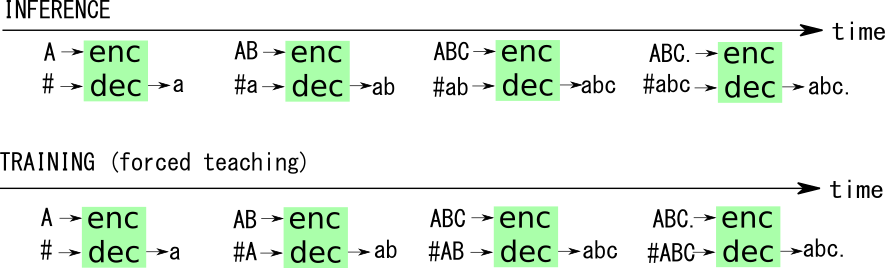
\includegraphics[width=6in]
{transformer/transformer-train-test.png}
\caption{Training and Inference for vanilla transformer.
``enc" and ``dec" denote
the encoder and decoder, respectively.
A hash character represents the SOS (start of sentence) token,
and a period represents the EOS (end of sentence) token. Capital letters represent ground
truth tokens, and lower case ones represent 
predictions.}
\label{fig-transformer-train-test}
\end{figure}

\item {\bf Masked Attention}

\beq
P(\alp|\nu, \alp') = 0 
\text{ if $\alp'>\alp$}
\eeq
$\alp$ and $\alp'$ are
sentence positions and $\alp'$ is the future of $\alp$.
So as to
not violate causality,
 do not pay attention to sentence positions in the future.



\end{itemize}

\subsection{Single Head Attention}
\begin{figure}[h!]\centering
\begin{minipage}{.5\linewidth}
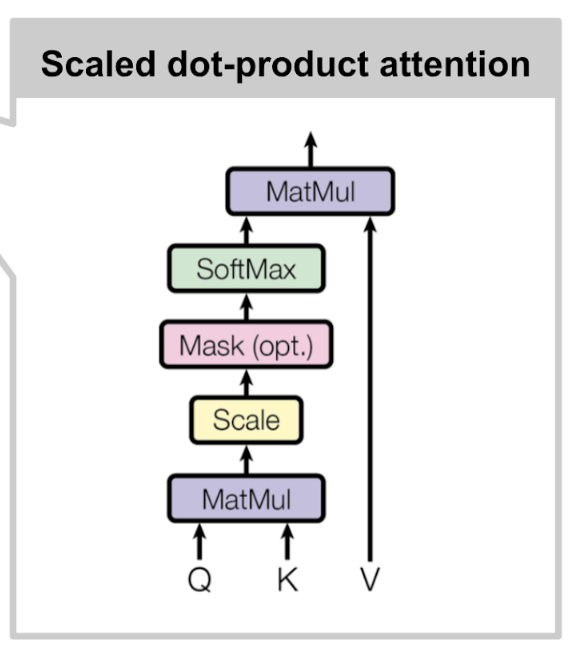
\includegraphics[width=2in]{transformer/scaled-dot-prod-att.jpg}
\end{minipage}%blank lines between minispaces breaks this
\begin{minipage}{.5\linewidth}
$$\xymatrix{
*+[F*:Orchid]{\underline{A}^{[d], [\ell]}}&&&
\\
&&*+[F*:SpringGreen]{\underline{P}^{[\ell], [\ell]}}\ar[ull]&
\\
&&*+[F*:Lavender]{\underline{M}^{[\ell], [\ell]}}\ar[u]&
\\
&&*+[F*:yellow]{\underline{S}^{[\ell],[\ell]}}\ar[u]&
\\
&&*+[F*:Orchid]{\underline{B}^{[\ell], [\ell]}}\ar[u]&
\\
*+[F*:Orchid]{\underline{V}^{[d],[\ell]}}\ar[uuuuu]&*+[F*:Orchid]{\underline{K}^{[d],[\ell]}}\ar[ur]&&*+[F*:Orchid]{\underline{Q}^{[d],[\ell]}}\ar[ul]
}$$
\end{minipage}
\caption{Scaled Dot Product Attention.}
\label{fig-texnn-for-scaled-dot-prod-att}
\end{figure}

\begin{subequations}

\begin{equation}\color{blue}
A^{[d], [\ell]} = V^{[d],[\ell]} P^{[\ell], [\ell]}\;\;\text{$\left(\text{Note that }\sum_{\alp\in[\ell]} P^{\alp, [\ell]}=1\right)$}
\label{eq-P-fun-scaled-dot-prod-att}
\end{equation}

\begin{equation}\color{blue}
B^{[\ell], [\ell]} = (K^{[d],[\ell]})^T Q^{[d],[\ell]}
\label{eq-B-fun-scaled-dot-prod-att}
\end{equation}

\begin{equation}\color{blue}
K^{[d],[\ell]} = \;\;\text{prior}
\label{eq-K-fun-scaled-dot-prod-att}
\end{equation}

\begin{equation}\color{blue}
M^{[\ell], [\ell]} = \text{mask}(S^{[\ell],[\ell]})
\label{eq-R-fun-scaled-dot-prod-att}
\end{equation}

\begin{equation}\color{blue}
P^{[\ell], [\ell]} = \text{softmax}(M^{[\ell], [\ell]})\;\;\text{$\left(\text{Note that }\sum_{\alp\in[\ell]} P^{\alp, [\ell]}=1\right)$}
\label{eq-G-fun-scaled-dot-prod-att}
\end{equation}

\begin{equation}\color{blue}
Q^{[d],[\ell]} = \;\;\text{prior}
\label{eq-Q-fun-scaled-dot-prod-att}
\end{equation}

\begin{equation}\color{blue}
S^{[\ell],[\ell]} = \frac{B^{[\ell], [\ell]}}{\sqrt{d}}
\label{eq-Y-fun-scaled-dot-prod-att}
\end{equation}

\begin{equation}\color{blue}
V^{[d],[\ell]} = \;\;\text{prior}
\label{eq-V-fun-scaled-dot-prod-att}
\end{equation}

\end{subequations}

\subsection{Multi-Head Attention}

\begin{figure}[h!]\centering
\begin{minipage}{.35\linewidth}
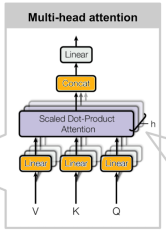
\includegraphics[width=2in]{transformer/multi-head-att.png}
\end{minipage}%blank lines between minispaces breaks this
\begin{minipage}{.65\linewidth}
$$\xymatrix@C=0.7pc{
&&*+[F*:Orchid]{\underline{Q_0}^{[d],[\ell]}}\ar[dddr]&&&
\\
&*+[F*:Dandelion]{\underline{Q}^{[D], [\ell]}}\ar[ur]\ar[dr]&&&&
\\
&&*+[F*:Orchid]{\underline{Q_1}^{[d],[\ell]}}\ar[dddr]&&&
\\
&&*+[F*:Orchid]{\underline{K_0}^{[d],[\ell]}}\ar[r]&*+[F*:Orchid]{\underline{A_0}^{[d],[\ell]}}\ar[dr]&&
\\
*+[F*:SpringGreen]{\underline{e}^{[d], [\ell]}}\ar[r]\ar[uuur]\ar[dddr]&*+[F*:Dandelion]{\underline{K}^{[D], [\ell]}}\ar[ur]\ar[dr]&&&*+[F*:yellow]{\underline{A}^{[D],[\ell]}}\ar[r]&*+[F*:Dandelion]{\underline{O}^{[d],[\ell]}}
\\
&&*+[F*:Orchid]{\underline{K_1}^{[d],[\ell]}}\ar[r]&*+[F*:Orchid]{\underline{A_1}^{[d],[\ell]}}\ar[ur]&&
\\
&&*+[F*:Orchid]{\underline{V_0}^{[d],[\ell]}}\ar[uuur]&&&
\\
&*+[F*:Dandelion]{\underline{V}^{[D], [\ell]}}\ar[ur]\ar[dr]&&&&
\\
&&*+[F*:Orchid]{\underline{V_1}^{[d],[\ell]}}\ar[uuur]&&&
}$$
\end{minipage}
\caption{Multi-head Attention with 2 heads.Note that the input $\rve$ and output $\underline{O}$ have the same shape.}
\label{fig-texnn-for-multi-head-att}
\end{figure}

\begin{subequations}

\begin{equation}\color{blue}
A^{[D],[\ell]} = [A_0^{[d],[\ell]}|A_1^{[d],[\ell]}]
\label{eq-C-fun-multi-head-att}
\end{equation}

\begin{equation}\color{blue}
A_0^{[d],[\ell]} = \text{scaled\_dot\_prod\_att}(Q_0^{[d],[\ell]},K_0^{[d],[\ell]},V_0^{[d],[\ell]})
\label{eq-X-fun-multi-head-att}
\end{equation}

\begin{equation}\color{blue}
A_1^{[d],[\ell]} = \text{scaled\_dot\_prod\_att}(Q_1^{[d],[\ell]},K_1^{[d],[\ell]},V_1^{[d],[\ell]})
\label{eq-Y-fun-multi-head-att}
\end{equation}

\begin{equation}\color{blue}
K^{[D], [\ell]} = W_\rvk^{[D],[d]}e^{[d], [\ell]}
\label{eq-K-fun-multi-head-att}
\end{equation}

\begin{equation}\color{blue}
K_0^{[d],[\ell]} = \text{linear}(K^{[D], [\ell]})\;\;\text{(split, then project a component)}
\label{eq-4-fun-multi-head-att}
\end{equation}

\begin{equation}\color{blue}
K_1^{[d],[\ell]} = \text{linear}(K^{[D], [\ell]})\;\;\text{(split, then project a component)}
\label{eq-5-fun-multi-head-att}
\end{equation}

\begin{equation}\color{blue}
O^{[d],[\ell]} = W_\rvo^{[d],[D]}A^{[D],[\ell]}
\label{eq-F-fun-multi-head-att}
\end{equation}

\begin{equation}\color{blue}
Q^{[D], [\ell]} = W_\rvq^{[D],[d]}e^{[d], [\ell]}
\label{eq-Q-fun-multi-head-att}
\end{equation}

\begin{equation}\color{blue}
Q_0^{[d],[\ell]} = \text{linear}(Q^{[D], [\ell]})\;\;\text{(split, then project a component)}
\label{eq-1-fun-multi-head-att}
\end{equation}

\begin{equation}\color{blue}
Q_1^{[d],[\ell]} = \text{linear}(Q^{[D], [\ell]})\;\;\text{(split, then project a component)}
\label{eq-2-fun-multi-head-att}
\end{equation}

\begin{equation}\color{blue}
V^{[D], [\ell]} = W_\rvv^{[D],[d]}e^{[d], [\ell]}
\label{eq-V-fun-multi-head-att}
\end{equation}

\begin{equation}\color{blue}
V_0^{[d],[\ell]} = \text{linear}(V^{[D], [\ell]})\;\;\text{(split, then project a component)}
\label{eq-7-fun-multi-head-att}
\end{equation}

\begin{equation}\color{blue}
V_1^{[d],[\ell]} = \text{linear}(V^{[D], [\ell]})\;\;\text{(split, then project a component)}
\label{eq-8-fun-multi-head-att}
\end{equation}

\begin{equation}\color{blue}
e^{[d], [\ell]} = \;\;\text{prior}
\label{eq-e-fun-multi-head-att}
\end{equation}

\end{subequations}

\subsection{Encoder}
\begin{figure}[h!]\centering
\begin{minipage}{.4\linewidth}
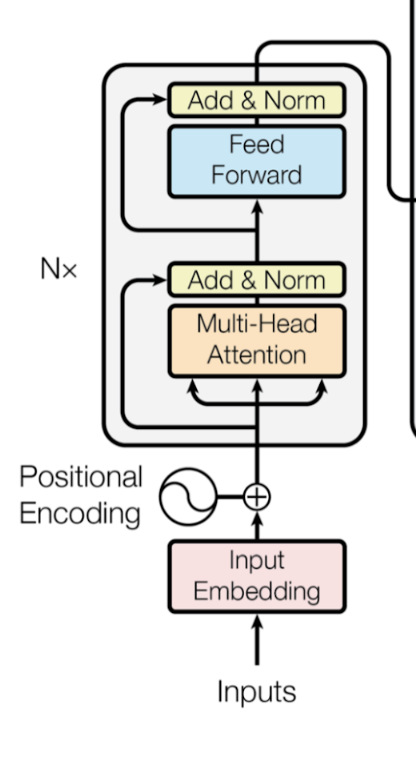
\includegraphics[width=2in]{transformer/encoder.jpg}
\end{minipage}%blank lines between minispaces breaks this
\begin{minipage}{.6\linewidth}
$$\xymatrix@R=2.5pc@C=0.1pc{
*+[F*:yellow]{\underline{n}^{[\Lambda],[d], [\ell]}}&&&
\\
&*+[F*:SkyBlue]{\underline{F}^{[\Lambda],[d], [\ell]}}\ar[ul]&&
\\
*+[F*:yellow]{\underline{N}^{[\Lambda],[d], [\ell]}}\ar[ur]\ar[uu]&&&
\\
&&*+[F*:Dandelion]{\underline{O}^{[\Lambda],[d], [\ell]}}\ar[ull]&
\\
&*+[F*:Dandelion]{\underline{Q}^{[\Lambda],[D], [\ell]}}\ar[ur]&*+[F*:Dandelion]{\underline{K}^{[\Lambda],[D], [\ell]}}\ar[u]&*+[F*:Dandelion]{\underline{V}^{[\Lambda],[D], [\ell]}}\ar[ul]
\\
*+[F*:gray]{\underline{e}^{[\Lambda],[d], [\ell]}}\ar[urr]\ar[uuu]\ar[ur]\ar[urrr]&&&
\\
*+[F*:Lavender]{\underline{x}^{[L],[\ell]}}\ar[u]&&&
\save
\POS"1,1"."6,1"."1,4"."6,4"!C*+<4.0em>\frm{-,}
\restore
\\
*+[F-,]{\;\;}&\text{$\Lambda$ layers}
}$$
\end{minipage}
\caption{Encoder.}
\label{fig-texnn-for-encoder}
\end{figure}

\begin{subequations}

\begin{equation}\color{blue}
F^{[\Lambda],[d], [\ell]} = \text{feed\_forward\_nn}(N^{[\Lambda],[d], [\ell]})
\label{eq-F-fun-encoder}
\end{equation}

\begin{equation}\color{blue}
K^{[\Lambda],[D], [\ell]} = W_\rvk^{[D], [d]}e^{[\Lambda],[d], [\ell]}
\label{eq-K-fun-encoder}
\end{equation}

\begin{equation}\color{blue}
N^{[\Lambda],[d], [\ell]} = \text{normalize}(e^{[\Lambda],[d], [\ell]} + O^{[\Lambda],[d], [\ell]})
\label{eq-N-fun-encoder}
\end{equation}

\begin{equation}\color{blue}
O^{[\Lambda],[d], [\ell]} = \text{multi\_headed\_attention}(Q^{[\Lambda],[D], [\ell]},K^{[\Lambda],[D], [\ell]},V^{[\Lambda],[D], [\ell]})
\label{eq-O-fun-encoder}
\end{equation}

\begin{equation}\color{blue}
Q^{[\Lambda],[D], [\ell]} = W_\rvq^{[D], [d]}e^{[\Lambda],[d], [\ell]}
\label{eq-Q-fun-encoder}
\end{equation}

\begin{equation}\color{blue}
V^{[\Lambda],[D], [\ell]} = W_\rvv^{[D], [d]}e^{[\Lambda],[d], [\ell]}
\label{eq-V-fun-encoder}
\end{equation}

\begin{equation}\color{blue}
e^{[\Lambda],[d], [\ell]} = E^{[\Lambda],[d], [L]}x^{[L],[\ell]}
\label{eq-p-fun-encoder}
\end{equation}

\begin{equation}\color{blue}
n^{[\Lambda],[d], [\ell]} = \text{normalize}(N^{[\Lambda],[d], [\ell]} + F^{[\Lambda],[d], [\ell]})
\label{eq-n-fun-encoder}
\end{equation}

\begin{equation}\color{blue}
x^{[L],[\ell]} = \;\;\text{prior}
\label{eq-R-fun-encoder}
\end{equation}

\end{subequations}



\subsection{Decoder}

\begin{figure}[h!]\centering
\begin{minipage}{.4\linewidth}
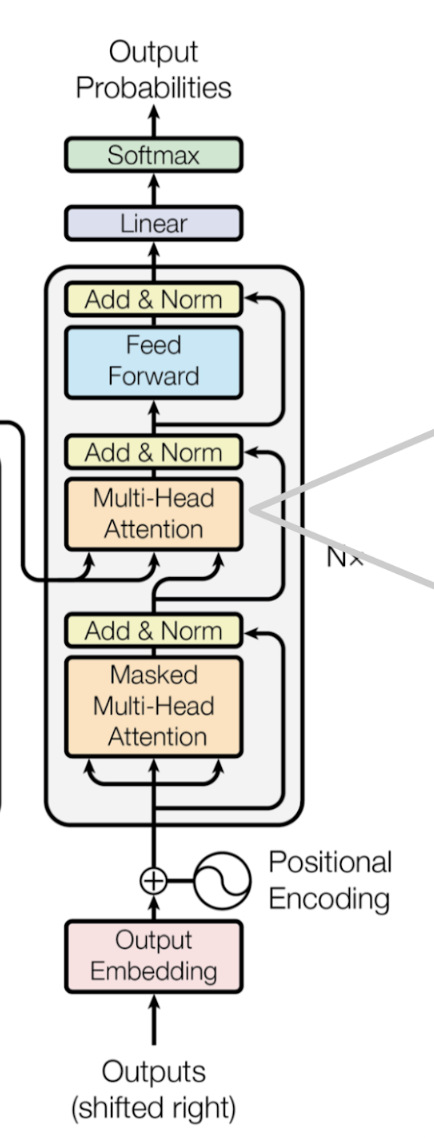
\includegraphics[width=2in]{transformer/decoder.jpg}
\end{minipage}%blank lines between minispaces breaks this
\begin{minipage}{.6\linewidth}
$$\xymatrix@R=2.5pc@C=0.2pc{
&&&*+[F*:SpringGreen]{\underline{P}^{[L],[\ell]}}
\\
&&&*+[F*:Orchid]{\underline{I}^{[L],[\ell]}}\ar[u]
\\
&&&*+[F*:yellow]{\underline{Y}^{[\Lambda],[d], [\ell]}}\ar[u]
\\
&&*+[F*:SkyBlue]{\underline{F}^{[\Lambda],[d], [\ell]}}\ar[ur]&
\\
&*+[F*:Dandelion]{\underline{o}^{[\Lambda],[d],[\ell]}}\ar[rr]&&*+[F*:yellow]{\underline{j}^{[\Lambda],[d], [\ell]}}\ar[ul]\ar[uu]
\\
*+[F*:Dandelion]{\underline{v}^{[\Lambda],[D], [\ell]}}\ar[ur]&*+[F*:Dandelion]{\underline{k}^{[\Lambda],[D], [\ell]}}\ar[u]&*+[F*:Dandelion]{\underline{q}^{[\Lambda],[D], [\ell]}}\ar[ul]&
\\
*+[F*:yellow]{\underline{n}^{[\Lambda],[D], [\ell]}}\ar[ur]\ar[u]&&&*+[F*:yellow]{\underline{a}^{[\Lambda],[d], [\ell]}}\ar[uu]\ar[ul]
\\
&*+[F*:Dandelion]{\underline{O}^{[\Lambda],[d],[\ell]}}\ar[urr]&&
\\
*+[F*:Dandelion]{\underline{Q}^{[\Lambda],[D], [\ell]}}\ar[ur]&*+[F*:Dandelion]{\underline{K}^{[\Lambda],[D], [\ell]}}\ar[u]&*+[F*:Dandelion]{\underline{V}^{[\Lambda],[D], [\ell]}}\ar[ul]&
\\
&&&*+[F*:gray]{\underline{e}^{[\Lambda],[d],[\ell]}}\ar[ull]\ar[ulll]\ar[ul]\ar[uuu]
\\
&&&*+[F*:Lavender]{\underline{x}^{[L],[\ell]}}\ar[u]
\save
\POS"3,1"."10,1"."3,4"."10,4"!C*+<4.0em>\frm{-,}
\restore
\\
*+[F-,]{\;\;}&\text{$\Lambda$ layers}
}$$
\end{minipage}
\caption{Decoder.}
\label{fig-texnn-for-decoder}
\end{figure}

\begin{subequations}

\begin{equation}\color{blue}
F^{[\Lambda],[d], [\ell]} = \text{feed\_forward\_nn}(j^{[\Lambda],[d], [\ell]})
\label{eq-B-fun-decoder}
\end{equation}

\begin{equation}\color{blue}
I^{[L],[\ell]} = W^{[L],[\Lambda], [d]}Y^{[\Lambda],[d], [\ell]}
\label{eq-I-fun-decoder}
\end{equation}

\begin{equation}\color{blue}
K^{[\Lambda],[D], [\ell]} = W_\rvk^{[D],[d]}e^{[\Lambda],[d],[\ell]}
\label{eq-K-fun-decoder}
\end{equation}

\begin{equation}\color{blue}
O^{[\Lambda],[d],[\ell]} = \text{multi\_head\_attention}(Q^{[\Lambda],[D], [\ell]},K^{[\Lambda],[D], [\ell]},V^{[\Lambda],[D], [\ell]})
\label{eq-o-fun-decoder}
\end{equation}

\begin{equation}\color{blue}
P^{[L],[\ell]} = \text{softmax}(I^{[L],[\ell]})\;\;\text{$(\sum_{\alp\in[\ell]}P^{[L], \alp}=1)$}
\label{eq-G-fun-decoder}
\end{equation}

\begin{equation}\color{blue}
Q^{[\Lambda],[D], [\ell]} = W_\rvq^{[D],[d]}e^{[\Lambda],[d],[\ell]}
\label{eq-Q-fun-decoder}
\end{equation}

\begin{equation}\color{blue}
V^{[\Lambda],[D], [\ell]} = W_\rvv^{[D],[d]}e^{[\Lambda],[d],[\ell]}
\label{eq-V-fun-decoder}
\end{equation}

\begin{equation}\color{blue}
Y^{[\Lambda],[d], [\ell]} = \text{normalize}(F^{[\Lambda],[d], [\ell]} + a^{[\Lambda],[d], [\ell]})
\label{eq-Y-fun-decoder}
\end{equation}

\begin{equation}\color{blue}
a^{[\Lambda],[d], [\ell]} = \text{normalize}(O^{[\Lambda],[d],[\ell]} + e^{[\Lambda],[d],[\ell]})
\label{eq-a-fun-decoder}
\end{equation}

\begin{equation}\color{blue}
e^{[\Lambda],[d],[\ell]} = E^{[\Lambda],[d],[L]}x^{[L],[\ell]}
\label{eq-p-fun-decoder}
\end{equation}

\begin{equation}\color{blue}
j^{[\Lambda],[d], [\ell]} = \text{normalize}(o^{[\Lambda],[d],[\ell]} + a^{[\Lambda],[d], [\ell]})
\label{eq-j-fun-decoder}
\end{equation}

\begin{equation}\color{blue}
k^{[\Lambda],[D], [\ell]} = U_\rvk^{[D],[d]}n^{[\Lambda],[D], [\ell]}
\label{eq-k-fun-decoder}
\end{equation}

\begin{equation}\color{blue}
n^{[\Lambda],[D], [\ell]} = \;\;\text{Prior comming from Encoder.}
\label{eq-n-fun-decoder}
\end{equation}

\begin{equation}\color{blue}
o^{[\Lambda],[d],[\ell]} = \text{multi\_head\_attention}(v^{[\Lambda],[D], [\ell]},k^{[\Lambda],[D], [\ell]},q^{[\Lambda],[D], [\ell]})
\label{eq-O-fun-decoder}
\end{equation}

\begin{equation}\color{blue}
q^{[\Lambda],[D], [\ell]} = U_\rvq^{[D],[d]}a^{[\Lambda],[d], [\ell]}
\label{eq-q-fun-decoder}
\end{equation}

\begin{equation}\color{blue}
v^{[\Lambda],[D], [\ell]} = U_\rvv^{[D], [d]}n^{[\Lambda],[D], [\ell]}
\label{eq-v-fun-decoder}
\end{equation}

\begin{equation}\color{blue}
x^{[L],[\ell]} = \;\;\text{prior}
\label{eq-R-fun-decoder}
\end{equation}

\end{subequations}